\section{Access control module}

\subsection{Problem Summary}

\hspace{0.35cm} Currently, the complete content offered in the courses on Bodhitree can be accessed by any student who is registered for the course. If a student has access to a course, the he has access to all the videos, documents, quizzes and assignments in that course.
\par There might be a case where the instructor wants to limit the access of content to the students. He might want some students to not have access to a particular content type, for example, the instructor would want only those students to have access to the in-video quizzes who have made some payment.
\par The access control module enables the instructor to provide differential access to students based upon the access that he grants them.

\subsection{Specifications}

The specifications were provided by the content developers which are meant to control the access that each individual student has to the content offered on Bodhitree. They are as follows:

\begin{enumerate}
	\item The instructor can tag the elements present in each concept. These elements can be any one of the following:
	\begin{enumerate}
		\item Videos
		\item Documents
		\item Quizzes
		\item Video Markers (In-video Quizzes)
	\end{enumerate}
	\item These tagged elements cannot be accessed by the students having the default access to Bodhitree, i.e. students having access only to the free content.
	\item Several elements can be tagged under one tag, for example, a video titled \textit{``HTML 5 Intro"} and a document titled \textit{``CSS \& Styles"} can be tagged as \textit{``P1"}. So, such elements come under a group which is denoted by a tag. The access to that particular tag denotes the access provided to those group of elements.
	\item A student not having access to a particular tagged element can still see the title and the link to open that element, but when he tries to access the element, a dialogue box is displayed which informs him that he does not have access to that element.
	\item In case of video markers: If the video markers are tagged and the student does not have access to that particular tag, then the video will be shown as a plain MP4 video without any in-video quizzes or information markers.
	\item The instructor can upload a CSV file which contains the username's of the students that are currently registered on Bodhitree followed by the tags that the instructors want the students to have access to. A sample CSV file is shown below:
	
	\begin{center}
		\begin{tabular}{|c|c|c|c|}
		\hline \rule[-2ex]{0pt}{5.5ex} stud1 & P1 & P2 & P3 \\ 
		\hline \rule[-2ex]{0pt}{5.5ex} stud2 & P1 &  &  \\ 
		\hline \rule[-2ex]{0pt}{5.5ex} stud3 & P3 &  &  \\ 
		\hline 
		\end{tabular} \\
		\vspace{0.2cm}
		\textit{Table 2}: Sample CSV file for uploading the students access tags
	\end{center}
	
	\item The students who have access to a particular tag can access all the elements that are marked by that tag.
\end{enumerate}

\subsection{System Design}

When an element (video, document or quiz) is created in a concept, the default tag is set as \textit{``Free''}. Video markers are also set as \textit{``Free"} when a video is created. The elements can then be tagged by the instructor/content developer by opening the page on which the element is displayed.

\subsubsection*{Tagging interface:}

\begin{figure}[h]
\centering
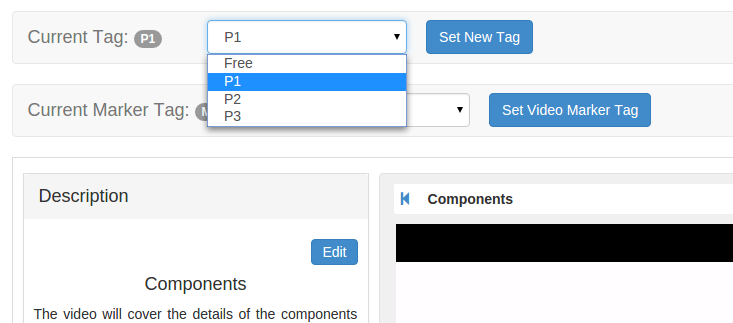
\includegraphics[width=1\linewidth]{./media/tagging_interface}
\caption{Tagging interface for video}
\label{fig:tagging_interface}
\end{figure}

\begin{enumerate}

	\item The tagging interface consists of the following:
	\begin{enumerate}
		\item A label \textit{``Current Tag:"} followed by a badge. The badge shows the current tag of the element.
		\item A drop down box which lists the 5 fixed tags \textit{(P1, P2, P3, P4, P5)}, as well as the custom tags set by the instructor.
		\item A button labelled \textit{``Set New Tag"}, on clicking it sets the new tag selected in the drop down box to that element.
	\end{enumerate}
	
	\item A field \textit{``premium\_tag"} was added in the database table of each element of a concept, namely, the video, quiz and document table. An additional field \textit{``premium\_marker"} was added in the video table which stores the tags of the video markers.
	
	\begin{figure}[h]
	\centering
	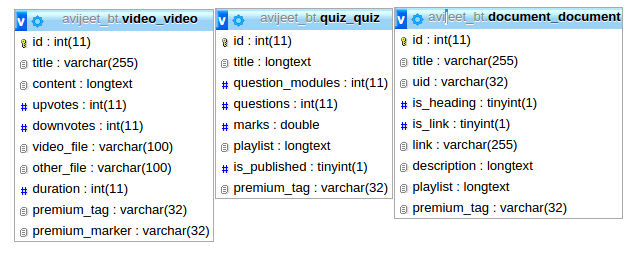
\includegraphics[width=0.9\linewidth]{./media/elementsSchema}
	\caption{Premium tags in the tables of Video, Quiz and Document}
	\label{fig:elementsSchema}
	\end{figure}

	\item Once a new tag has been set to the element, the \textit{premium\_tag} field in the table of that element changes to the new tag.
	
\end{enumerate}

\subsubsection*{Student's view:}

\begin{enumerate}
	\item Any student who has registered for the course can view all the elements that are tagged \textit{``Free"}.
	
	\item If a student tries to access an element that has been tagged and if he has not been given access to that tag, then instead of showing that element, an information box is shown which displays that the user does not have access to the content and a link is shown using which the student can use to request access to the content. It is depicted in the figure below:
	\begin{figure}[h]
		\centering
		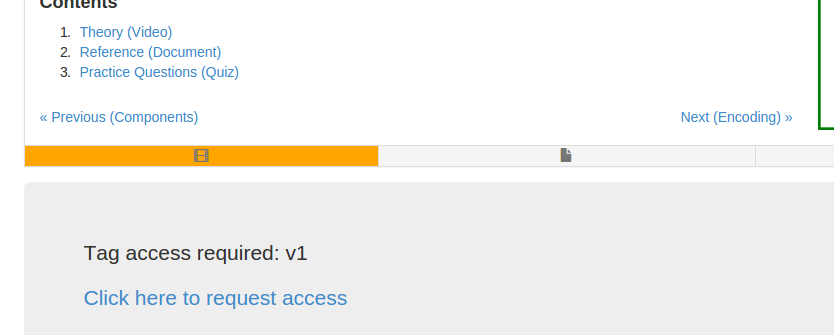
\includegraphics[width=0.8\linewidth]{./media/sAccessNot}
		\caption{An Uunauthorized student trying to view a tagged content}
		\label{fig:sAccessNot}
	\end{figure}
	
	\item When a user opens a concept page, the tags he has access to is checked from the \textit{premiumuser} table, that is shown in \textit{Figure 8}.

	\item The data of only those elements of the concept is fetched from the database to whom the user has access to. For the rest of the elements, the key value pair \textit{has\_access} is \textit{false}.
	
	\item If the value of \textit{has\_access} is \textit{false}, then the element is not shown to the user. The following figures show the data that is fetched to the client to implement access control.
	
	\item The first \textit{Figure 8} shows that the user does not have access to the element. Hence, the \textit{``has\_access"} and \textit{``marker\_access"} is \textit{false}. Also note that the markers list is empty, as the user does not have access to the video markers.
	
	\item Note that the \textit{``video\_file"} url and the \textit{``other\_file"} url data is not displayed to the user not having access to the corresponding tag.
	
	\begin{figure}[h]
	\centering
	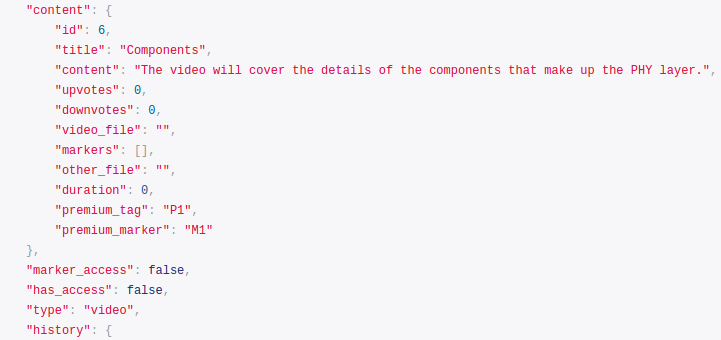
\includegraphics[width=1\linewidth]{./media/SUgetdata}
	\caption{Data sent to user not having access to the element}
	\label{fig:SUgetdata}
	\end{figure}

	\item The second \textit{Figure 9} shows that the user has access to the element. Hence, the \textit{``has\_access"} and \textit{``marker\_access"} is \textit{true} and all the required data is fetched from the server to display the element.
	
	\item Note that when the user has access, the complete data including the markers, video duration, other files details and the video file url is sent to the client.

	\begin{figure}
	\centering
	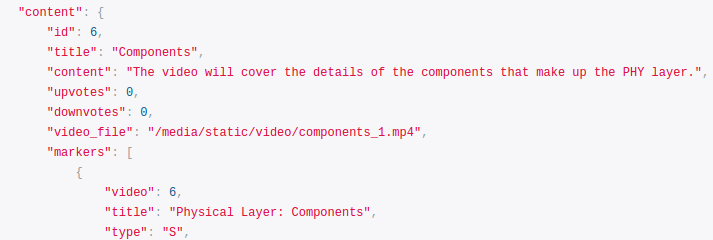
\includegraphics[width=1\linewidth]{./media/SAgetdata1}
	. \\
	. \\
	. \\
	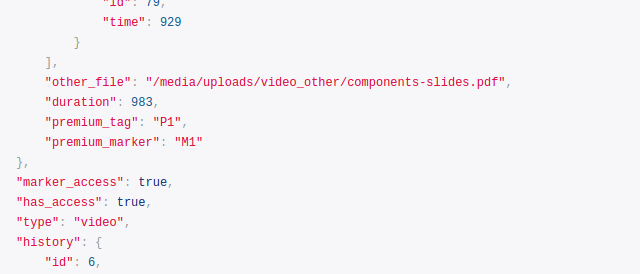
\includegraphics[width=1\linewidth]{./media/SAgetdata2}
	\caption{Data sent to the user having access to the element}
	\label{fig:SAgetdata2}
	\end{figure}

\end{enumerate}

\newpage

\subsubsection*{Providing tag access to students:}

\begin{enumerate}
	\item The instructor uploads a CSV file as shown in Table 2.
	\item Each username is checked against the users registered in Bodhitree.
	\item If the user is valid, then an entry is added in the database table \textit{``premiumuser"} which has the following three fields:
	\begin{enumerate}
		\item Username \textit{(user\_id)}
		\item ID of the current course \textit{(course\_id)}
		\item Premium tag name \textit{(premium\_type)}
	\end{enumerate}
	\item This table stores the tag accesses each user has been provided for a particular course.
	
	\begin{figure}[h]
	\centering
	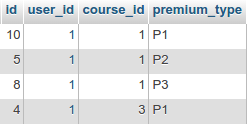
\includegraphics[width=0.4\linewidth]{./media/premiumAccesses}
	\caption{Snapshot of the database table which stores the user access to tags}
	\label{fig:premiumAccesses}
	\end{figure}
	
	\item If the username is not found, then it is indicated to the instructor after he uploads the CSV file. Also, the current user accesses are also displayed to the instructor on the CSV uploading page, as shown in \textit{Figure 11}.
	
	\item On successful upload of the CSV file having the user accesses to tags, an information page is displayed which shows the following details:
	
	\begin{enumerate}
		\item \textit{Existing premium users}: The users which already have access to certain tags.
		\item \textit{Users added as premium}: The new users/tags which were added to \textit{premiumuser} table.
		\item \textit{Unknown users}: The users which are mentioned in the CSV file but who are not registered on Bodhitree.
	\end{enumerate}
		
	\textit{Figure 12} depicts the successful upload information of the CSV.
	
\end{enumerate}

\begin{figure}
\centering
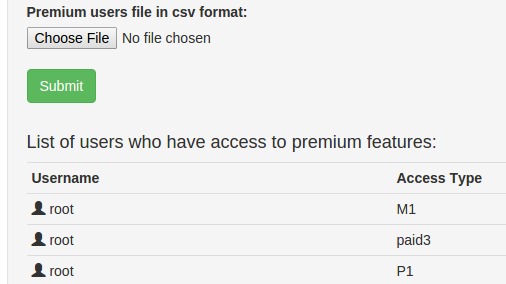
\includegraphics[width=0.7\linewidth]{./media/CSVupload}
\caption{Interface to upload the CSV file containing the user accesses to tags}
\label{fig:CSVupload}
\vspace{1cm}
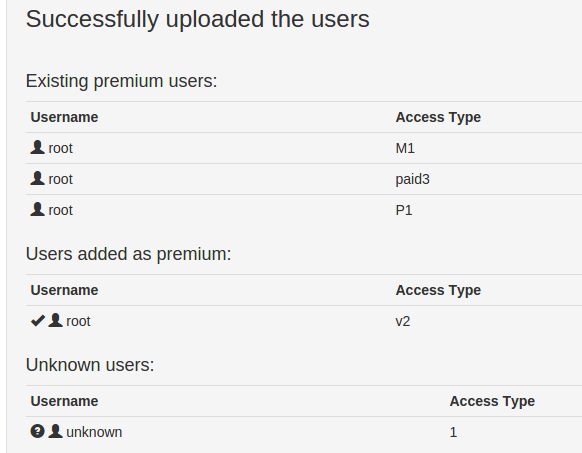
\includegraphics[width=0.7\linewidth]{./media/usertaguploadsuccess}
\caption{Information displayed after successfully uploading the CSV file}
\label{fig:usertaguploadsuccess}
\end{figure}

\subsubsection*{Removal of access to tags from users:}

\begin{enumerate}
	\item An interface is displayed to the instructor which shows the current users and the associated tags to which they have access to.
	\item It is displayed in the form of a checklist, wherein the instructor can check the users and the tag access which he wants to remove and then clicking on the delete button provided will remove the corresponding entries from the database, stripping those users from the access to those tags. The users then are no longer able to access the elements corresponding to those tags.
\end{enumerate}

\begin{figure}[h]
\centering
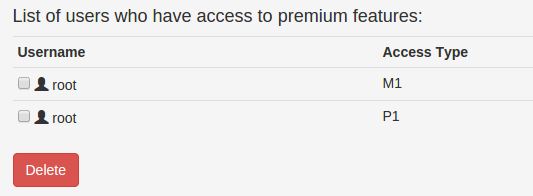
\includegraphics[width=0.8\linewidth]{./media/removeusers}
\caption{Interface to remove user access to tags}
\label{fig:removeusers}
\end{figure}

\subsubsection*{Handling authorization:}

\begin{enumerate}
	\item Only the Instructor ot the Content Developer must be able to grant access to other users. No unauthorized user should be able to access the CSV upload page of the Access Control module. This is done by displaying an unauthorized access page to the student who is trying to access the instructor page.
	\item A user who does not have access to a particular tag must not be able to access any element associated with that tag. This is achieved by checking the authorization when the data is generated at the server side and sending only that data to the client to which he has access to.
	\item Only the Instructor or Content Developer must be able to set the tag to an element. This is achieved by not displaying the element tagging area to any user who is not an Instructor or Content Developer.
\end{enumerate}

%\subsection{Future Work}